
%(BEGIN_QUESTION)
% Copyright 2010, Tony R. Kuphaldt, released under the Creative Commons Attribution License (v 1.0)
% This means you may do almost anything with this work of mine, so long as you give me proper credit

A newly constructed PLC-controlled motor starter system refuses to work -- the motor shaft does not turn after the operator presses the ``Start'' switch and waits.  After this, you measure 0 volts AC between the terminals labeled ``C'' and ``D'' on the Stop switch.  A laptop PC shows the PLC program as it exists in memory, but without any colored status highlighting:

$$\includegraphics[width=15.5cm]{i03661x01.eps}$$

Identify the likelihood of each specified fault in this system.  Consider each fault one at a time (i.e. no coincidental faults), determining whether or not each fault could independently account for {\it all} measurements and symptoms in this circuit.

% No blank lines allowed between lines of an \halign structure!
% I use comments (%) instead, so that TeX doesn't choke.

$$\vbox{\offinterlineskip
\halign{\strut
\vrule \quad\hfil # \ \hfil & 
\vrule \quad\hfil # \ \hfil & 
\vrule \quad\hfil # \ \hfil \vrule \cr
\noalign{\hrule}
%
% First row
{\bf Fault} & {\bf Possible} & {\bf Impossible} \cr
%
\noalign{\hrule}
%
% Another row
Start pushbutton switch failed open &  &  \cr
%
\noalign{\hrule}
%
% Another row
Stop pushbutton switch failed open &  &  \cr
%
\noalign{\hrule}
%
% Another row
Open wire between L1 and junction block &  &  \cr
%
\noalign{\hrule}
%
% Another row
Thermal overload tripped &  &  \cr
%
\noalign{\hrule}
%
% Another row
Open wire between L1 and TRIAC card Common &  &  \cr
%
\noalign{\hrule}
%
% Another row
Blown ``L1'' 480 VAC fuse &  &  \cr
%
\noalign{\hrule}
} % End of \halign 
}$$ % End of \vbox

\underbar{file i03661}
%(END_QUESTION)





%(BEGIN_ANSWER)

% No blank lines allowed between lines of an \halign structure!
% I use comments (%) instead, so that TeX doesn't choke.

$$\vbox{\offinterlineskip
\halign{\strut
\vrule \quad\hfil # \ \hfil & 
\vrule \quad\hfil # \ \hfil & 
\vrule \quad\hfil # \ \hfil \vrule \cr
\noalign{\hrule}
%
% First row
{\bf Fault} & {\bf Possible} & {\bf Impossible} \cr
%
\noalign{\hrule}
%
% Another row
Start pushbutton switch failed open & $\surd$ &  \cr
%
\noalign{\hrule}
%
% Another row
Stop pushbutton switch failed open &  & $\surd$ \cr
%
\noalign{\hrule}
%
% Another row
Open wire between L1 and junction block & $\surd$ &  \cr
%
\noalign{\hrule}
%
% Another row
Thermal overload tripped & $\surd$ &  \cr
%
\noalign{\hrule}
%
% Another row
Open wire between L1 and TRIAC card Common & $\surd$ &  \cr
%
\noalign{\hrule}
%
% Another row
Blown ``L1'' 480 VAC fuse & $\surd$ &  \cr
%
\noalign{\hrule}
} % End of \halign 
}$$ % End of \vbox

%(END_ANSWER)





%(BEGIN_NOTES)

{\bf This question is intended for exams only and not worksheets!}.

%(END_NOTES)

